% ****** Start of file apssamp.tex ******
%
%   This file is part of the APS files in the REVTeX 4 distribution.
%   Version 4.0 of REVTeX, August 2001
%
%   Copyright (c) 2001 The American Physical Society.
%
%   See the REVTeX 4 README file for restrictions and more information.
%
% TeX'ing this file requires that you have AMS-LaTeX 2.0 installed
% as well as the rest of the prerequisites for REVTeX 4.0
%
% See the REVTeX 4 README file
% It also requires running BibTeX. The commands are as follows:
%
%  1)  latex apssamp.tex
%  2)  bibtex apssampya
%  3)  latex apssamp.tex
%  4)  latex apssamp.tex
%
%\documentclass[preprint, pra,groupedaddress,amsmath,amssymb, onecolumn]{revtex4}
\documentclass[preprint, prX, amsmath,amssymb]{revtex4-1}


\setlength{\parindent}{10mm}
%\documentclass[twocolumn,pra,groupedaddress,amsmath,amssymb]{revtex4}
%\documentclass[twocolumn,pra,showpacs,groupedaddress,superscriptaddress,amsmath,amssymb]{revtex4}
%\documentclass[preprint,showpacs,preprintnumbers,amsmath,amssymb]{revtex4}

% Some other (several out of many) possibilities
%\documentclass[preprint,aps]{revtex4}
%\documentclass[preprint,aps,draft]{revtex4}
%\documentclass[pra]{revtex4}% Physical Review B

\usepackage{graphicx}% Include figure files
\usepackage{braket}
\usepackage{amsmath}
\usepackage{bm}% bold math
\usepackage[latin1]{inputenc}
\usepackage{subfig} 
\usepackage{listings}
\lstset{language=C}

%\usepackage{dcolumn}% Align table columns on decimal point

\begin{document}

\title{CME213	Final Project Report}
	
\author{Dong-Bang Tsai}
	\email{dbtsai@stanford.edu}
	\affiliation{Stanford University, Stanford, California 94305, USA}
%\date{\today}% It is always \today, today,

\begin{abstract}
In this final project of CME213, we were given a problem which is similar to sparse matrix vector multiplication, but not exactly the same in order to demonstrate the ability for us to implement and optimize the algorithm for given problem. I'll discuss about how do I  solve this problem.

After doing the analysis of this problem, I found that it can be recast into segmented scan problem. Although segmented scan can be easily parallelized as work-efficient algorithm using CPU implementation, it's not the case in the GPU implementation. The NVIDIA GPU architecture executes the threads of a block in SIMT (single instruction, multiple thread) groups of 32 called warps, the threads of a warp may follow any execution path, and they execute with a shared instruction unit and thus are executing only a single instruction at any instant in time; therefore, it's inefficient that each thread in a block takes care of one segment, and loops all the element in the segment. Also, even all the threads in one wrap can run different instructions, the memory access pattern is still irregular, so the performance is not good according to my experiment. 

Another way to implement the segmented scan in parallel is reduce/downsweep method scanning in the wrap which is mentioned in the class, but the work complexity is twice compared with Intra-Warp Scan Algorithm\cite{Shubhabrata2008}. In the reference\cite{Shubhabrata2008}, they claimed that reduce/downsweep leads to measurably lower performance compared with Intra-Warp Scan Algorithm.

To sum up, my final implementation use Intra-Warp Scan Algorithm to scan each segment. As a result, each segment will be assigned to dedicated warp to perform the inclusive scan, and in each time, a warp will process 31 elements. In next step, the wrap will move on to next 31 elements, and process them. This approach will lead to good memory access pattern. However, if the segments are less than the total concurrent warps, which are $16 * 48 = 768$ for GTX 580,  then not all the processing power will be utilized, and this is something I can improve in the future. 

\end{abstract}

\maketitle



\section{The given problem}

The following input data will be given:
\begin{itemize}
\item Sequence $a_0,\dots, a_{n-1}$
\item Segments $s_0, \dots, s_{p-1}$ such that $s_0=0$, $s_{p-1}=n$, and $s_{j-1}<s_j$ for all $0<j<p$.
\item Sequence $x_0, \dots, x_{q-1}$
\item Sequence $k_0, \dots, k_{n-1}$ such that $0\leq k_l <q$
\end{itemize}
We want to compute the following:
\begin{align}
    b_j=\sum_{l=si}^j a_l x_{k_l}, \text{ for all } 0\le j<n,\;s_i\le j<s_{i+1}\label{eq:ME}
\end{align}

Since we want to perform this calculation repeatedly many times, and update $a$ using $b$ at each step, in a manner similar to an iterative method that computes matrix-vector products, which is
\begin{align}
   &1)\; b_j=\sum_{l=si}^j a_l x_{k_l}, \text{ for all } 0\le j<n,\;s_i\le j<s_{i+1}\label{eq:ME}\\
   &2)\; a = b.
\end{align}

If we take closer look at $x$, we will find that in each iterative step, the value is not changed at all. Although we can use permutation iterator to access the $x$ vector through the $k$ mapping vector, the memory access patten is not coalesced; therefore, we can simply define a bigger vector $\bar{x}_l = x_{k_l}$, which will be used through all the iterations. Since $a_l\bar{x}_l$ for all $l$ needed to be calculated, here I use the transform function in thrust library. 

One tricky thing here, when we do the summation (segmented scan), actually we can do in-memory computation, it implies that we don't need to do ping-pong here, and only needs one array.

To sum up, the algorithm for this problem will be three steps as the following.
\begin{itemize}
\item 1) Flatten the $x_{k_l}$ vector into $\bar{x}_l$ vector to increase the memory coalesce.   
\item 2) Perform the transformation $a_l \doteq a_l\bar{x}_l$ for all $l$.
\item 3) Perform in-memory segmented scan $a_l \doteq \sum_{l=s_i}^j a_l$, and repeat from 2)
\end{itemize}

\section{Correctness Test reference and CPU implementation}

I  checked the result using both \textbf{referencesp\_MVscan-released.cu} and my own CPU implementation, the relative errors are all smaller than $10^{-6}$ for three steps. Since I already have the report in the first submission, I don't attach it here in order to save some space. In my CPU implementation, I  use openMP to parallelize the transformation and segmented scan. Since there is no wrap issue in CPU, each thread will take care of one segment. Once finished, just move on to another unfinished segment. 

\begin{lstlisting}
        cpu_buffer.resize(n);
        thrust::copy(a.begin(), a.end(), cpu_buffer.begin());
        cpu_curr = &cpu_buffer[0];        
        cpu_start_time = omp_get_wtime(); 
        for(int iter=0; iter<iters;++iter)
        {  
             // Perform the step 2) in algorithm
            #pragma omp parallel for 
            for(int i=0; i<n; ++i){ cpu_curr[i] *= xx[i];}
            // Perform the step 3), segmented scan in CPU
            #pragma omp parallel for 
            for(int i=1; i<p; ++i)
                for(int j=s[i-1]+1; j<s[i]; ++j) 
                  cpu_curr[j] += cpu_curr[j-1]; 
        }
        cpu_end_time = omp_get_wtime();
\end{lstlisting}

The CPU implementation has good scaling when I increased the \# of processors, and it's almost linear from 1 to 4 CPUs. The performance of CPU implementation is given in Fig.~(\ref{CPU}). When the \# of threads are more than 8, in some case, the performance will be decreased. The reason may be memory bank-conflict. I don't have time to address this issue.
\begin{figure}
  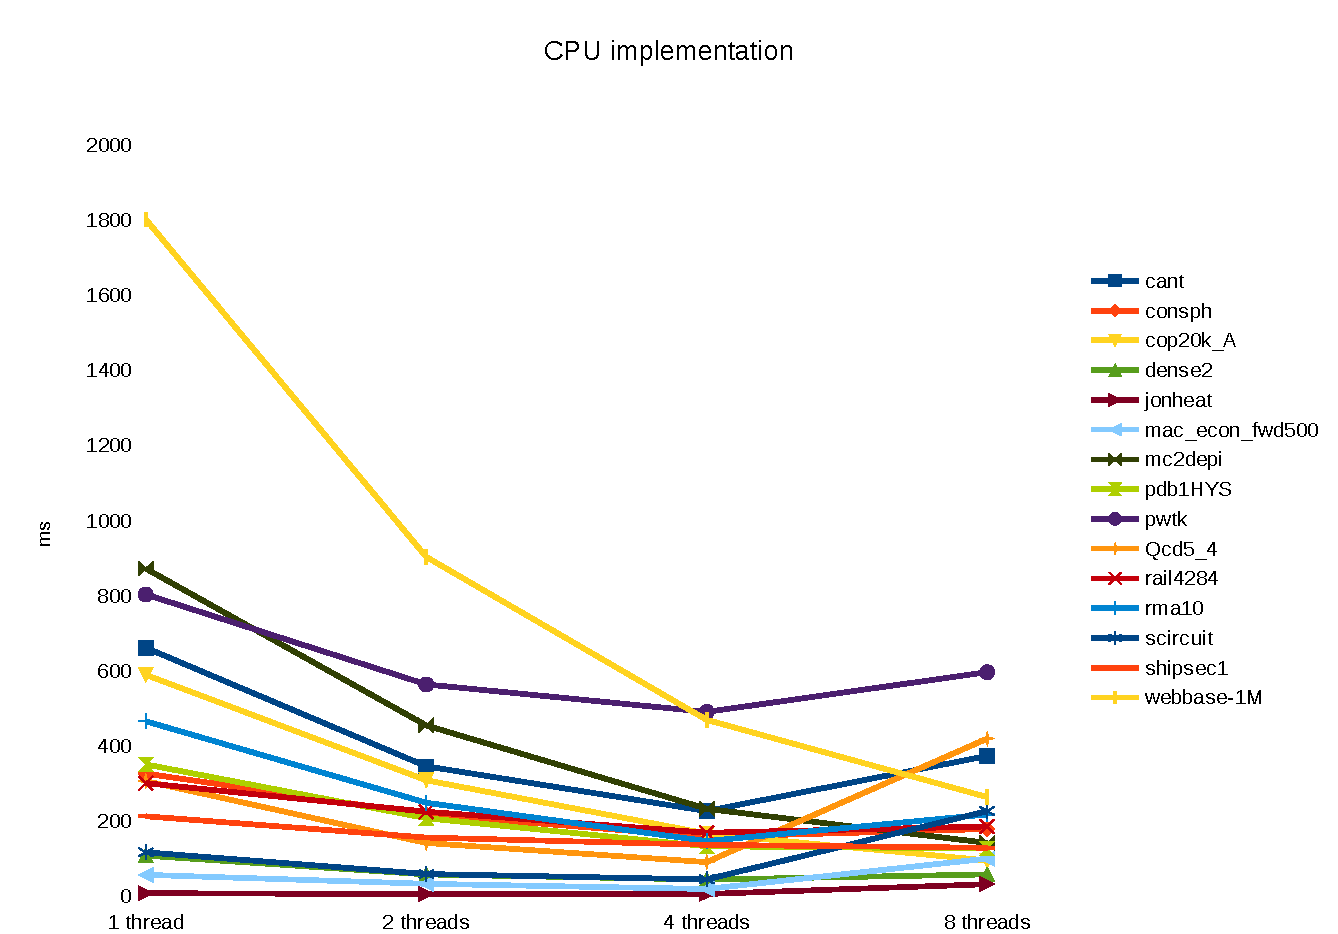
\includegraphics[width=15.2cm]{CPU}\\
\caption{OpenMP CPU implementation.}
\label{CPU}

\end{figure}


\section{Naive GPU implementation}

The following is my first naive GPU implementation submitted on Friday. Here, I do three tests. The first one is only one thread in a wrap doing work, and each thread is dedicated to one segment. Thus, the memory access patten is coalesce, but only one thread out of 32 is working. The second test is that the first thread in half wrap is doing work; therefore, there are two threads working in one wrap. Each thread also works on one segment. The last experiment are all the threads in the wraps are enabled.

\begin{lstlisting}
template<typename floatType>
__global__
void SegmentedScan(floatType *curr, floatType *xx, int* s, int p, int threads)
{
    int thread_id = threadIdx.x + (blockIdx.y * gridDim.x + blockIdx.x) *
                              blockDim.x; // global thread index
    // global warp index, from 1 to p-1
    int warp_id = thread_id / threads + 1;
    // thread index within the warp
    int lane = thread_id & (threads - 1); 

    if(warp_id < p && lane ==0)
    {
        int start = s[warp_id-1];
        int end = s[warp_id];
        curr[start] = prev[start];
        for(int j=start+1; j<end; ++j){  curr[j] += curr[j-1]; }
    }
}

// Main Code
    for(int iter=0; iter<iters;++iter)
    { 
        thrust::transform(gpu_curr, gpu_curr+n, xx_gpu.begin(), 
            gpu_curr, thrust::multiplies<GPUFloatType>());
        SegmentedScan<GPUFloatType><<<blocks, threads>>>
           (thrust::raw_pointer_cast(gpu_curr), 
            thrust::raw_pointer_cast(&xx_gpu[0]), 
            thrust::raw_pointer_cast(&s_gpu[0]), p, threads_in_segment);
    }

\end{lstlisting}

\begin{figure}
  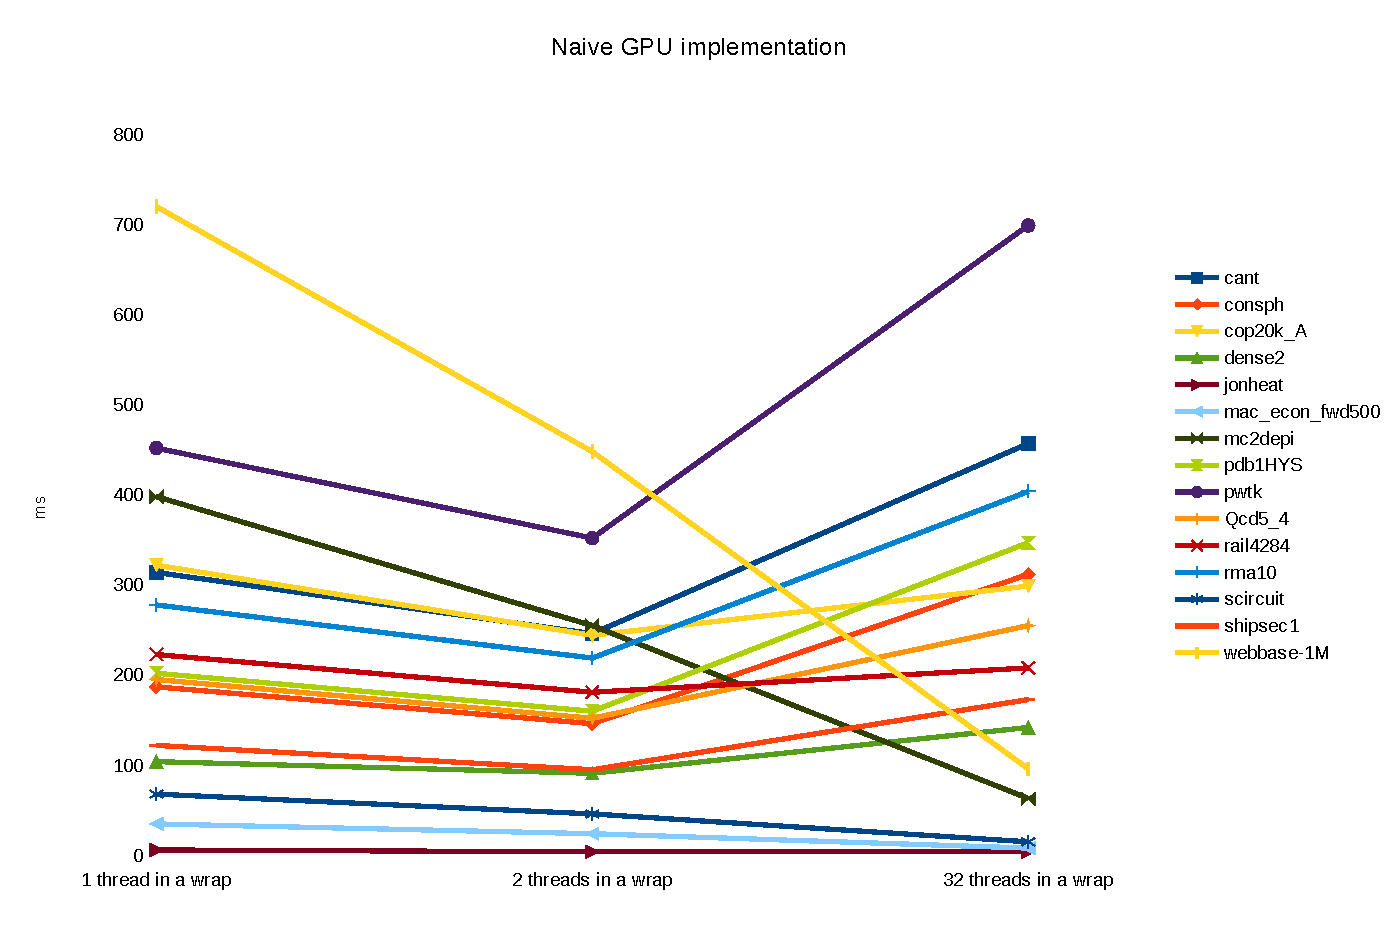
\includegraphics[width=15.2cm]{GPU1}\\
\caption{Naive GPU implementation.}
\label{GPU1}
\end{figure}

The result of naive GPU implementation is very interesting. As you can see in the Fig.~(\ref{GPU1}), for most of the cases, when half wrap is working on one segment will give the best performance. The reason is in Nvidia GPU, the memory access operation will be performed and grouped together with the unit of half wrap. Therefore, when 32 threads in a warp are computing different part of segments, the memory cache performance will be decreased due to the irregular access pattern. However, for webbase-1M and pwtk, even we use all the threads in a warp, the performances still are not decreased. The reason is for those two cases, each segment has small numbers of elements; therefore, when 32 threads start to process segment $p$ to $p+31$, the memory addresses are still near each other; therefore, the low-performance impact from irregular access will be lower.

\section{Final implementation, Intra-Warp Scan Algorithm}

As we know that NVIDIA GPU executes the threads of block in SIMT groups of 32 called wraps, we can use this property of synchronous execution of threads in a warp to eliminate the need for barriers. Take closer look at the following code, we don't need barriers for synchronous, and it will run the same instruction, read, write to memory at the same time across all the threads in a wrap.  Since we want to use 32 threads at one time to compute 32 elements, we can also unroll the loop to increase the performance. Here, for each 32 elements, the complexity of this is $O(w\log w) = O(32\log32)$; however, since the threads of a warp execute in SIMT way, if we try to decrease the $w$ to decrease the overhead, for example, using $w=8$, then we may need more steps and also cause the irregular memory access patten. But, in presumption, I'll say that maybe using $w=16$ can decrease the overhead, and also avoid the irregular memory access problem. This is something I didn't try but would like to figure out in the future. Note that, the first thread actually always does nothing in the inclusive sum; as a result, in each step, we just move forward for 31 elements. 

\begin{lstlisting}

template<typename floatType>
__device__
void scan_warp ( floatType * curr , const unsigned int lane, 
                  const unsigned int start, const unsigned int end )
{
    if ( lane >= 1  && start+lane < end)  
        curr[start+lane] = curr[start+lane-1 ] + curr[start+lane];
    if ( lane >= 2  && start+lane < end)  
        curr[start+lane] = curr[start+lane-2 ] + curr[start+lane]; 
    if ( lane >= 4  && start+lane < end)  
        curr[start+lane] = curr[start+lane-4 ] + curr[start+lane];
    if ( lane >= 8  && start+lane < end)  
        curr[start+lane] = curr[start+lane-8 ] + curr[start+lane];
    if ( lane >= 16 && start+lane < end)  
        curr[start+lane] = curr[start+lane-16] + curr[start+lane];
}

template<typename floatType>
__global__
void SegmentedScan(floatType *curr, floatType *xx, int* s, int p, int threads)
{
  // global thread index
    int thread_id = threadIdx.x + (blockIdx.y * gridDim.x + blockIdx.x) 
    * blockDim.x; 
    // global warp index, from 1 to p-1
    int warp_id = thread_id / threads + 1;
     // thread index within the warp
    int lane = thread_id & (threads - 1);

    if(warp_id < p)
    {
        int start = s[warp_id-1];
        int end = s[warp_id];

        while(start < end)
        {
            scan_warp(&curr[0], lane, start, end);
            start += 31;
        }
    }
}
\end{lstlisting}

The Fig.~(\ref{Final}) demonstrates the result of Intra-Wrap Scan method, and they are almost the fastest compared with naive implementation. Some of the cases have lower performance in intra-warp scan compared with in naive implementation. For example, webbase-1M has this problem; the reason is that for those cases which have smaller number of elements in one segment, using 32 threads to do intra-wrap scan is inefficient. 

\begin{figure}
  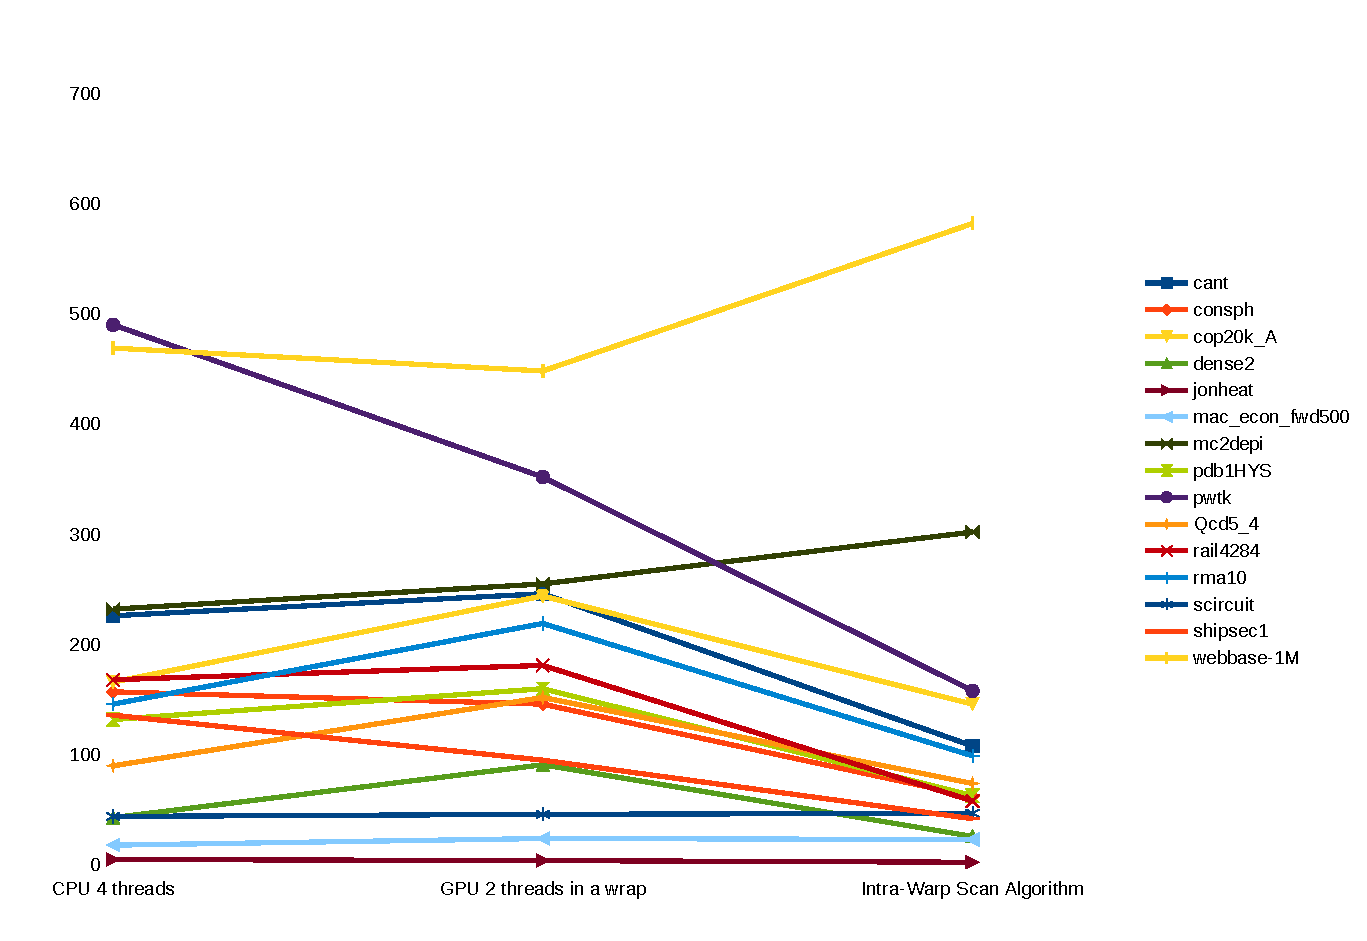
\includegraphics[width=15.2cm]{Final}\\
\caption{OpenMP 4 threads, Naive 2 threads in a wrap, and Intra-Wrap Scan.}
\label{Final}
\end{figure}

The following is the raw data for Intra-Warp Scan Algorithm.\\
cant: The running time of my code for 50 iterations is: 107.911 milliseconds. \\
consph: The running time of my code for 20 iterations is: 62.1167 milliseconds.\\ 
cop20k\_A: The running time of my code for 73 iterations is: 146.603 milliseconds.\\
dense2: The running time of my code for 10 iterations is: 26.6759 milliseconds. \\
jonheart: The running time of my code for 60 iterations is: 2.66506 milliseconds. \\
mac\_econ\_fwd500: The running time of my code for 12 iterations is: 23.5443 milliseconds.\\ 
mc2depi: The running time of my code for 70 iterations is: 302.068 milliseconds. \\
pdb1HYS: The running time of my code for 30 iterations is: 63.5818 milliseconds. \\
pwtk: The running time of my code for 25 iterations is: 158.697 milliseconds. \\
qcd5\_4: The running time of my code for 63 iterations is: 74.6078 milliseconds.\\ 
rail4284: The running time of my code for 10 iterations is: 58.7522 milliseconds. \\
rma10: The running time of my code for 74 iterations is: 99.9466 milliseconds. \\
scircuit: The running time of my code for 30 iterations is: 47.8156 milliseconds. \\
shipsec1: The running time of my code for 10 iterations is: 42.4012 milliseconds. \\
webbase-1M: The running time of my code for 77 iterations is: 592.115 milliseconds. 

\section{Conclusion}
The GPU is designed for regular execution path, i.e., SIMT fashion, and regular memory access patterns, i.e., memory coalescing; therefore, the Intra-Warp Scan Algorithm is the best fitted algorithm in GPU as I already demonstrated. The work I'll like to try in the future will be 1) Verify if performance of reduce/downsweep algorithm is lower than Intra-Warp Scan Algorithm. and 2) Implement the half wrap per segment version of Intra-Warp Scan Algorithm to decrease the overhead.  We demonstrated that the memory access unit in CUDA is half wrap; therefore, we should be able to decrease the overhead without causing the irregular memory access patterns. 

\begin{references}
\bibitem{Shubhabrata2008} Shubhabrata Sengupta
, Mark Harris, and Michael Garland, ``Efficient Parallel Scan Algorithms for GPUs'',  NVIDIA Technical Report NVR-2008-003, December (2008)
    \end{references}
\end{document}


